% This is part of Un soupçon de mathématique sans être agressif pour autant
% Copyright (c) 2015
%   Laurent Claessens
% See the file fdl-1.3.txt for copying conditions.

\begin{exercice}\label{exo2smath-0167}

    Le drapeau de la République Tchèque est comme ceci :
    %\begin{center}
    %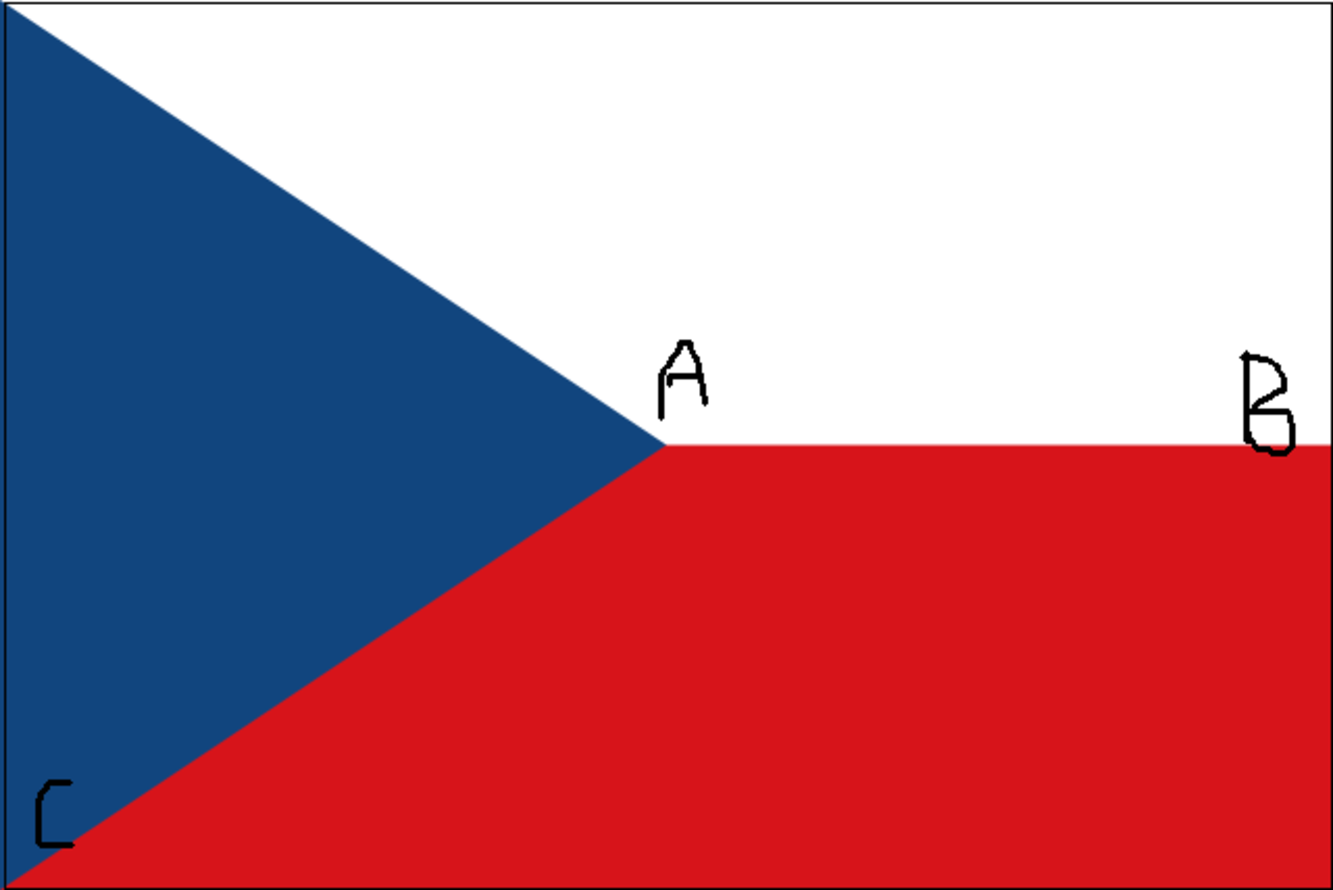
\includegraphics[width=5cm]{Czech_Republic.pdf}
    %\end{center}
    \begin{center}
\input{Fig_LLBQooAjaorQ.pstricks}
    \end{center}
    Sachant que l'angle de la partie bleue en \( E\) mesure \SI{70}{\degree}, déterminer les deux autres angles de sommet \( E\).
    
    Aide : une façon de faire est de suivre les étapes suivantes :
    \begin{enumerate}
        \item
            Déterminer les angles en \( A\) et \( B\).
        \item
            Prolonger le segment \( [DE]\) et nommer \( K\) le point d'intersection avec \( (AB)\).
        \item
            Déterminer les angles en \( K\).
    \end{enumerate}
    
\corrref{2smath-0167}
\end{exercice}
